\section{The Standard Model}
\label{sec:sm}
The behaviour of fundamental particles and forces are described by the \sm of
particle physics, which was concocted in the 1970s, when the Higgs
mechanism was incorporated into Glashow's electroweak theory by Salam and Weinberg.
The theory prescribes a treatment
as to how fundamental particles interact via three of the four
fundamental forces, namely: the strong, weak and electromagnetic forces.

Mathematically, the \sm is a locally gauge invariant quantum field theory.
It inhabits a space-time with a global Poincar\'e symmetry that obeys a local
$SU_C(3)\otimes SU_L(2)\otimes U_Y(1)$ symmetry\footnote{
The convention of natural units is used throughout.
Other conventions are that the indices $\mu$ and $\nu$ are used for four vectors, and generators
for the $SU_L(2)$ and $SU_C(2)$ are denoted by $\{i,j,k\}$ and $\{a,b,c\}$, respectively.}.
The $SU_L(2)\otimes U_Y(1)$ gauge group contains the electroweak formalism, and the $SU_C(3)$ group
contains that of the strong force.
%Each generator in this group corresponds to a spin-1 gauge-boson;
%the $SU_C(3)$ group is obeyed by the strong force in the theory of \QCD,
%while the electroweak sector obeys the $SU_L(2)\otimes U_Y(1)$ gauge group.
Generators for each group correspond to the vector bosons which mediate
interactions ---
the $3+1$ electroweak gauge bosons ($Z$, $W^\pm$ and the photon), and
the eight gluons of the strong force.
A summary of gauge bosons in the \sm is given in \Tab{tab:sm:gauge}.


\begin{table}
  \caption[Fundamental, force-mediating, gauge bosons]
  {
    Fundamental, force-mediating, gauge bosons in the \sm.
    All values are taken from Ref.~\protect\cite{PDG2014}.
  }
  \label{tab:sm:gauge}
  \begin{center}
    \begin{tabular}{ccrc}
      \toprule
      Force
      & Particle & \cellc{Mass}  & Charge\\
      \midrule
      Electromagnetic & $\gamma$ & $0\phantom{\gev}$ & $\phantom{-}0$ \\
      \multirow{2}{*}{Weak} & $W^\pm$ & $80.4\gev$ & $\pm1$ \\
      & $Z$ & $90.2\gev$ & $\phantom{-}0$ \\
      Strong & $G^a$ & $0\phantom{\gev}$ & $\phantom{-}0$ \\
      \bottomrule
    \end{tabular}
  \end{center}
\end{table}


Symmetries are fundamental to the dynamics of particle physics.
It was shown by Emmy Noether that for each symmetry in the action of a physical system there is a
conserved quantity~\cite{Noether}.
This is Noether's theorem.
For any sensible theory of physics, it is necessary that the laws remain the same independent of
time and space, these symmetries lead to the conservations of momentum and energy, respectively.
Discrete symmetries of important are \gls{T} and \gls{P}, so that physics occurs the same
regardless of the direction of time, and under reflections in space.

%Noether -> Symmetries
%C P T

Spin-$\tfrac12$ particles in the \sm are known as fermions, and
are described by spinor fields, $\psi$, and obey the Dirac equation:
\begin{equation}
  \big(i\gamma^\mu\partial_\mu - m\big)\psi = 0.
  \label{th:eq:dirac}
\end{equation}
The fermions of the \sm can be broadly categorized into those which couple to the strong force,
\emph{quarks}, and those which do not, \emph{leptons}.
There are six quarks: up, down, charm, strange, top, and bottom (\uquark, \dquark, \cquark,
\squark, \tquark and \bquark); and six leptons:
the electronic leptons ($\nu_e$, $e$),
the muonic leptons ($\nu_\mu$, $\mu$),
and the tauonic leptons ($\nu_\tau$, $\tau$).
Due to the properties of the strong force, quarks can only be observed as colour-neutral bound
states, usually these are
\emph{mesons} (quark-antiquark bound states) and \emph{baryons} (bound states of three quarks).
%the electron, muon, tau ($e$, $\mu$, $\tau$), and
%their corresponding neutrinos ($\nu_e$, $\nu_\mu$, $\nu_\tau$).
All fermions are organized into pairs forming three generations.
%The fermions of the \sm constitute six leptons (electron, electron neutrino, muon, muon neutrino,
%tau and tau neutrino) and six quarks ($u$p, $d$own, $c$harm, $s$trange, $t$op and $b$ottom), which
%are organized into pairs forming three generations.
For each fermion there is a corresponding antiparticle with the same mass and opposite charge ---
charge being the conserved quantity resulting from the global electroweak gauge symmetry by
Noether's theorem.
A summary of all fermions and some of their properties is given in \Tab{tab:sm:particles}.
There is also a single scalar field in the \sm: the Higgs boson.
%The only additional particle is the scalar Higgs boson.

\begin{table}
  \caption[Fundamental fermions of matter]{
    Fundamental fermions of matter.
    In the \sm each has a corresponding anti-particle of opposite charge.
    All values are taken from Ref.~\protect\cite{PDG2014}.
  }
  \label{tab:sm:particles}
  \begin{center}
    \begin{tabular}{ccrccrc}
      \toprule
      & \multicolumn{3}{c}{Leptons}
      & \multicolumn{3}{c}{Quarks} \\
      Generation
    & Particle & \cellc{Mass}  & Charge
    & Particle & \cellc{Mass}  & Charge\\
      \midrule
      \multirow{2}{*}{1} & \ep   & $0.511\mev$ & $-1$ & \uquark & $2.3\mev$ & $+^2/_3$ \\
      & \neue & $0\phantom{\mev}$  &  $\phantom{-}0$ & \dquark & $4.8\mev$ & $-^1/_3$ \\
      \multirow{2}{*}{2} & \mup   & $0.105\gev$ & $-1$ & \cquark & $95.0\mev$ & $+^2/_3$ \\
      & \neum & $0\phantom{\mev}$  &  $\phantom{-}0$ & \squark & $1.275\gev$ & $-^1/_3$ \\
      \multirow{2}{*}{3} & \taup   & $1.777\gev$ & $-1$ & \tquark & $173\gev$ & $+^2/_3$ \\
      & \neut & $0\phantom{\mev}$  &  $\phantom{-}0$ & \bquark & $4.18\gev$ & $-^1/_3$ \\
      \bottomrule
    \end{tabular}
  \end{center}
\end{table}



The \sm Lagrangian can be expressed as a sum of components:
\begin{equation}
  \Lag{SM} = \Lag{QCD} + \Lag{V} + \Lag{\ell} + \Lag{\it q} + \Lag{Higgs} + \Lag{Yuk}.
  \label{eq:th:lag}
\end{equation}
These Lagrangians describe the:
strong force interactions between colour carrying particles in the theory of \QCD
(\Lag{QCD});
weak vector self-interactions (\Lag{V});
electroweak behaviour of leptons (\Lag{\ell});
electroweak behaviour of quarks (\Lag{\it q});
Higgs interaction (\Lag{Higgs}); and
Yukawa couplings (\Lag{Yuk}).

As well as the discrete symmetries of \gls{P} and \gls{T}, there is also the \gls{C} symmetry.
The violation of these symmetries are of fundamental interest
to modern particle physics.
%It is expected that the combined $C\!PT$ symmetry is conserved, but other symmetries can be
%violated, measurements
%It is kk
%The combined \CP symmetry is
%The
%The latter three terms of \Eq{eq:th:lag} (\Lag{\it q}, (\Lag{Higgs}, and \Lag{Yuk}) are of
%fundamental importance as
%to how flavour, and \CP violation arise in the \sm, and will be discussed in detail.
%There are three fundamental discrete symmetries in the \sm: \gls{C}, \gls{P}, and \gls{T}.
Violation of the combined \CP symmetry, and flavour, arise in the \ckm matrix of the \sm, which emerges
after the Higgs mechanism breaks the local electroweak symmetry.
The important terms for this are \Lag{\it q}, (\Lag{Higgs}, and \Lag{Yuk} from \Eq{eq:th:lag}.

The Higgs doublet, $\Phi$, is defined to be
\begin{equation}
  \Phi = \frac{1}{\sqrt{2}}
  \begin{pmatrix}
    \phi_1 + i\phi_2 \\
    \phi_3 + i\phi_4 \\
  \end{pmatrix},
  \label{eq:th:phi}
\end{equation}
where each $\phi_i$ is a real field.
The Lagrangian of the Higgs field is:
\begin{align}
  \Lag{Higgs}
  &= \big(D_\mu\Phi\big)^\dagger\big(D^\mu\Phi\big) - V\big(\Phi\big) \nonumber\\
  &= \big(D_\mu\Phi\big)^\dagger\big(D^\mu\Phi\big) - \mu^2\big(\Phi^\dagger\Phi\big) +
  \lambda\big(\Phi^\dagger\Phi\big)^{2},
  \label{eq:th:laghiggs1}
\end{align}
where $\mu$ and $\lambda$ are constants, and $D_\mu$ is the covariant derivative.
Figure~\ref{fig:th:higgspot} shows that
taking $\mu^2<0$ and $\lambda>0$ shifts the ground state of the vacuum of $V(\Phi)$ away from zero.
When the system collapses in to the ground state a direction is chosen, this breaks the symmetry of
the system.
%as shown in \Fig{fig:th:higgspot},
%shifts the minimum of the potential $V(\Phi)$ away from zero by a
The amount by which the ground state shifts with respect to the origin is
\begin{equation}
  v = \sqrt{\frac{\mu^2}{\lambda}}.
\end{equation}
At this point the Higgs field gets a \VEV of $\langle\phi\rangle = v/\sqrt{2}$.
%$\braket{\phi} = \tfrac{1}{\sqrt{2}}v$.
The direction of the \VEV from the origin is arbitrary, but the choice of
\begin{align}
  \bra{0}\phi_1\ket{0} =
  \bra{0}\phi_2\ket{0} =
  \bra{0}\phi_4\ket{0} &= 0 \nonumber\\
  \bra{0}\phi_3\ket{0} &= v,
\end{align}
is convenient, and changes the Higgs doublet in \Eq{eq:th:phi} to
\begin{equation}
  \Phi = \frac{1}{\sqrt{2}}
  \begin{pmatrix}
    \eta_1 + i\eta_2 \\
    v + i\eta_4 \\
  \end{pmatrix}.
  \label{eq:th:eta}
\end{equation}
Here, $\eta_1$, $\eta_2$ and $\eta_4$, are Goldstone bosons which, by choosing an appropriate
gauge, become the longitudinal components of the weak vector bosons, and $\Phi$ simplifies to
\begin{equation}
  \Phi = \frac{1}{\sqrt{2}}
  \begin{pmatrix} 0 \\ v+H
  \end{pmatrix},
  \label{eq:th:phi2}
\end{equation}
where $H$ is the physical Higgs boson.
Inserting Eq.~\ref{eq:th:phi2} into Eq.~\ref{eq:th:laghiggs1} gives:
%\begin{multline}
  %\Lag{Higgs} =
  %\frac12\left(\partial_\mu H\right)\left(\partial^\mu H\right)
  %+\frac14g^2\left(v^2 + 2vH + H^2\right)W_\mu^+W^{-\mu}  \\
  %+\frac18\left(g^2 + g^{\prime2}\right)\left(v^2 + 2vH + H^2\right)Z_\mu Z^\mu
  %+ \mu^2H^2 + \frac14\lambda\left(H^4+4vH^3\right) + \cdots,
  %\label{eq:th:laghiggs2}
%\end{multline}
\begin{equation}
  \Lag{Higgs} =
  \frac{1}{2}\big(\partial_\mu H\big)\big(\partial^\mu H\big)
  %+\mu^2H^2
  +\frac{m_H^2}{2}H^2
  +\left(m_W^2W_\mu^+W^{-\mu} + \frac{m_Z^2}{2}Z_\mu Z^\mu\right)
  %\cdot
  \left(1 + \frac{H}{v}\right)^{\!2}.
  \label{eq:th:laghiggs2}
\end{equation}
%where $g$ and $g^\prime$ are coupling constants and other terms are three- and four-point
%interactions of the Higgs with itself and weak gauge bosons.
Thus, there is \SSB of the local $U_Y(1)$ gauge group.
A result of this is that weak gauge bosons become massive, while photons remain massless: as is
consistent with observations.

\begin{figure}
  \begin{center}
    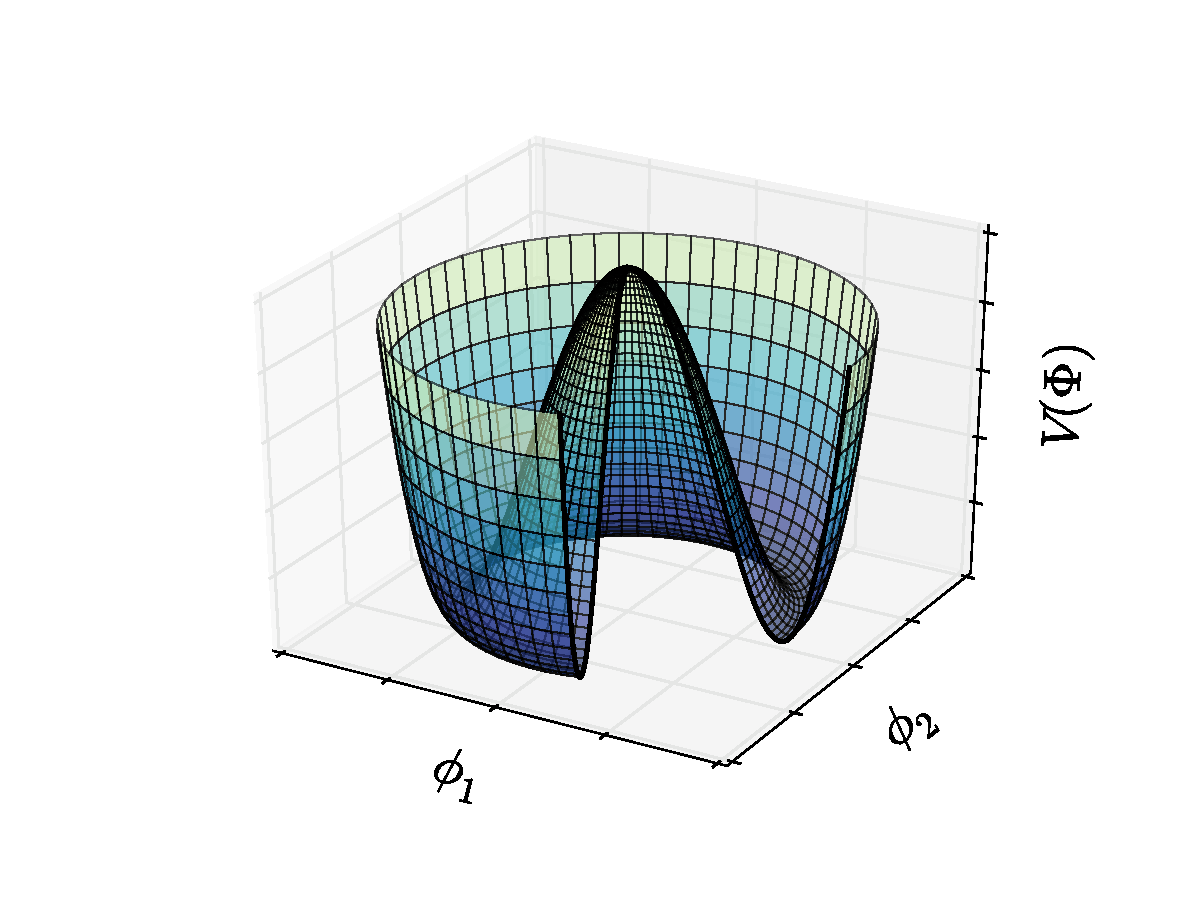
\includegraphics[width=0.6\textwidth]{higgs_potential}
    \caption[Shape of the Higgs potential]
    {
      The shape of the Higgs potential, $V(\Phi)$, for the simple case of $\Phi=\phi_1+i\phi_2$ and
      $\mu^2<0$ and $\lambda>0$.
      Spontaneous symmetry breaking occurs when the vacuum settles in a minima, and this choice of
      direction breaks the symmetry of the gauge.
      A section of the potential is not shown, to convey the shape of the potential.
    }
    \label{fig:th:higgspot}
  \end{center}
\end{figure}

All fermions (excepting neutrinos) also acquire mass after \SSB.
The Dirac mass term for a chiral field has the form:
\begin{equation}
  \Lag{mass} = -m_\psi\big(\xbar\psi_R\psi_L + \xbar\psi_L\psi_R\big),
  \label{eq:diracmass}
\end{equation}
but the left- and right-handed fields
($\psi_L$ and $\psi_R$) have different $U_Y(1)$ charges and so transform differently.
Using \Eq{eq:diracmass} to give masses to fermions would therefore break gauge invariance.
%and so cannot be added to \Lag{SM} without destroying the gauge invariance, hence \Eq{eq:diracmass}
%cannot be used.
Instead, masses are generated through the Yukawa couplings, which
describe interactions between all fermionic fields and the Higgs doublet.
This can be written
\begin{equation}
  %\Lag{Yuk} = \sum_{\substack{\ell=\\e,\mu,\tau}}\big(\Lag{Yuk}^\ell\big) + \Lag{Yuk}^q,
  \Lag{Yuk} = \sum_{\ell}\big(\Lag{Yuk}^\ell\big) + \Lag{Yuk}^q,
  \label{eq:th:yukking}
\end{equation}
where terms encapsulate lepton and quark interactions, respectively.
%where $\ell$ and $q$ denote the lepton and quark interactions, respectively.
Each lepton term describes the interaction between the Higgs boson and the chiral fields
$\ell_R$ and the spinor
\begin{align}
  \chi_L = \begin{pmatrix}\nu_L \\ \ell_L \end{pmatrix},
\end{align}
via
\begin{equation}
  \Lag{Yuk}^\ell
  = - g_\ell\big(\xbar\chi_L\Phi \ell_R + \xbar \ell_R\Phi^\dagger\chi_L\big),
\end{equation}
where each $g_\ell$ is a coupling constant.
After \SSB the Lagrangian becomes
\begin{align}
  \Lag{Yuk}^\ell
  = - m_\ell \big(\xbar\ell_L\ell_R + \xbar\ell_R\ell_L\big)%\cdot
  \left(1 + \frac{H}{v}\right)
\end{align}
and the lepton masses
\begin{equation}
  m_\ell = \frac{v}{\sqrt{2}}g_\ell
  \label{eq:leptonmass}
\end{equation}
are dependent on the fundamental parameters $g_\ell$ and $v$.

Yukawa interactions for quarks involve the right-handed chiral operators of the up- and down-type
quarks, $q_R^i$ for $q\in\{u,d\}$, and the left-handed doublet
\begin{equation}
  Q_L^i = \begin{pmatrix}u^i_L\\d^i_L\end{pmatrix}.
\end{equation}
Before \SSB, the Yukawa Lagrangian is
\begin{equation}
  \Lag{Yuk}^q = - y_{ij}^u\Xbar{Q}_L^i\Phi u_R^j
  - y_{ij}^d\Xbar{Q}_L^i\widetilde\Phi d_R^j +\,\mathrm{h.c.}
  \label{eq:th:lagyukq}
\end{equation}
where $\widetilde\Phi_i = \varepsilon_{ij}\Phi_k$, there is an implicit sum over the generations
$i$ and $j$, and the shorthand h.c.~denotes hermitian conjugate.
The coupling constants, $y^{q}$, are $3\times3$ matrices characterizing Yukawa coupling strengths
between generations.
After \SSB, $\Lag{Yuk}^q$ becomes:
\begin{equation}
  \Lag{Yuk}^q =
  - \frac{v}{\sqrt{2}}
  \left(
  y_{ij}^\uquark\uquarkbar_L^i\uquark_R^j
  + y_{ij}^\dquark\dquarkbar_L^i\dquark_R^j
  +\,\mathrm{h.c.}
  \right)
  %\cdot
  \left(1 + \frac{H}{v}\right).
  \label{eq:th:lagyuk2}
\end{equation}
Similar to lepton masses, in \Eq{eq:leptonmass}, quark masses are defined as
\begin{align}
  m_{ij}^u &= \frac{v}{\sqrt{2}}y_{ij}^u \nonumber\\
  m_{ij}^d &= \frac{v}{\sqrt{2}}y_{ij}^d.
\end{align}
Thus far, the flavour basis has been used, but it is now more convenient to change to the mass
basis, in which the matrices $m^{u,d}$ are diagonal., it is more convenient to change to a basis in which the matrix $m^q$
is diagonal, using the rotation matrices $V_L$ and $V_R$, such that
\begin{align}
  {m_{il}^{u}}^\prime &=  \big(V_L^{u\dagger}\big)_{ij} m_{jk}^u\big(V_R^u\big)_{kl} \nonumber\\
  {m_{il}^{d}}^\prime &=  \big(V_L^{d\dagger}\big)_{ij} m_{jk}^d\big(V_R^d\big)_{kl}.
\end{align}
The addition of a prime distinguishes the mass basis from the flavour basis.
This transformation is exactly equivalent to transforming the up- and
down-type chiral quark fields according to:
\begin{align}
  q_L^\prime &= \big(V_L^q\big)q_{L}^{} \nonumber\\
  q_R^\prime &= \big(V_R^q\big)q_{R}^{}.
\end{align}
Applying these transformations to all parts of \Lag{SM} leaves the majority of it unchanged, since
$V_{L}^{q\dagger} V_{L}^{q} = V_{R}^{q\dagger} V_{R}^{q} = \mathds{1}$ by definition.
%$m_{ij}^\mathrm{diag} = V_{Lik}m_{kl}(V_R^\dagger)_{lj}$.
%This is exactly equivalent to transforming the chiral quark fields for up- and down-type quarks
%accordingly:
%\begin{align}
  %q_L^\alpha = \left(V_L^q\right)_{\alpha i}q_L &&
  %q_R^\alpha = \left(V_R^q\right)_{\alpha i}q_R,
%\end{align}
%where the index of the original basis is identified with $i$ and the mass basis uses $\alpha$.
%The rotations of the basis of the chiral quark fields leave much of \Lag{SM} unchanged since
%$V_{qL}^\dagger V_{qL} = V_{qR}^\dagger V_{qR} = \mathbb{1}$.
However, this is not the case for \Lag{\it q}.

The Lagrangian $\Lag{\it q}$ can be decomposed into
$\Lag{\it q}^\mathrm{NC}+\Lag{\it q}^\mathrm{CC}$, where the
superscripts denote \NC and charged current \CC components.
The \NC part of the Lagrangian characterizes interactions between quarks and the neutral electroweak
vector bosons, while the \CC part involves the interactions of quarks wiht the charged $W^\pm$
bosons.
After changing to the mass basis, \Lag{NC} remains unchanged, whereas \Lag{CC}
transforms as:
\begin{align}
  \Lag{\it q}^\mathrm{CC}
  &= i\frac{g}{2}\gamma^\mu
  \bigg[\uquarkbar_Ld_LW^+_\mu + \dquarkbar_Lu_LW^-_\mu
  \bigg]  \nonumber\\
  &= i\frac{g}{2}\gamma^\mu
  \bigg[
    \uquarkbar_L^\prime\left(V_{uL}^{\phantom{\dagger}}V_{dL}^\dagger\right)d_L^{\,\prime} W^+_\mu +
    \dquarkbar_L^{\,\prime}\left(V_{dL}^{\phantom{\dagger}}V_{uL}^\dagger\right)u_L^\prime W^-_\mu
  \bigg]  \nonumber\\
  &= i\frac{g}{2}\gamma^\mu
  \bigg[
    \VCKM\uquarkbar_L^\prime d_L^{\,\prime} W^+_\mu +
    \VCKMconj\dquarkbar_L^{\,\prime} u_L^\prime W^-_\mu
  \bigg].
\end{align}
In the final step the matrix
$\VCKM=V^{\phantom{\dagger}}_{uL}V_{dL}^\dagger$ is defined.
This is known as the \ckm
matrix, and parameterizes the couplings between up- and down-type quarks in charged weak currents.



